\documentclass{article}
\usepackage{tikz,natbib} 
\title{Baroclinic Instabilities} 
\author{Jacob Perez} 
\begin{document} 
\maketitle
\tableofcontents 
\section{Introduction} 

Baroclinic instability is a fluid dynamical instability that occurs in stably stratified, rotating fluids. They are used to explain the generation and growth of extratropical cyclones. The main source of a baroclinic instability is caused by vertical shear of the background wind profile. On Earth this shearing is generated through the differential heating of the Earth from Sun causing a temperature gradient between the pole and equator. The existence of a meridional temperature gradient indicates a source of available potential energy (APE) released into the flow. The process of converting the APE produced from the meridional temperature gradient into kinetic energy (KE) is the essence of baroclinic instability.  

\subsection{Basic Mechanism} 

To make this idea clearer, a qualitative description of this process is given by \cite{Pedlosky1979}. In figure \ref{pedloskyexample} below we have the following situation, a constant potential temperature ($\theta_*$) surface tilts upward in the meridional plane by an angle $\alpha$. This creates a meridional the meridional temperature gradient. Now consider a fluid parcel starting at position A, be displaced to position B. By considering the change in density when moving from A to B, the restoring force becomes  
\begin{equation}
  E_* = \frac{g}{\theta_*}\frac{\partial\theta_*}{\partial z_*}\sin\phi\left[d_{z_*}-d_{y_*}\left(\frac{\partial z_*}{\partial y_*}\right)_{\theta_*}\right]
\end{equation}
where $d_{y_*}$ and $d_{z_*}$ are displacements in the $y$ and $z$ planes respectively and $\phi=\tan^{-1}(d_{z_*}/d_{y_*})$ is the angle of displacement. From this we can deduce that any vertical displacement ($d_{y_*}=0$ and $\sin\phi = 1$) reduces $E_*$ to the Brunt-V\"as\"al\"a frequency. For positive restoring forces we see that the system will return to an equilibrium state, but for a negative restoring force occurring when the fluid element satisfies
\begin{equation}
  0 < \tan\phi < \left(\frac{\partial z_*}{\partial y_*}\right),
\end{equation}
will cause the buoyancy force to accelerate the fluid parcel further and further away from its initial position. This is the main idea behind a baroclinic instability. For the fluid within this section defined by the angle $\phi$, the lower density fluid will rise, and the higher density fluid will sink, in turn releasing potential energy. The idea of varying densities can be directly linked variations in temperature of the fluid, meaning that a baroclinic instability is a form of thermal convection.

\begin{figure}[hb]
  \centering
  \begin{tikzpicture}
\draw[->,thick] (-5,0)--(5,0) node[right]{$y_*$};
\draw[->,thick] (0,-5)--(0,5) node[above]{$z_*$};
\draw[thick, rotate around = {315:(0,0)}] (4,-0.5) rectangle (-4,0.5) node[above]{$\theta_*$};
\fill (1.5,-1) circle [radius=2pt] node[below]{$A$};
\fill (-2.5,1) circle [radius=2pt] node[left] {$B$};
\draw (1.5,-1) -- (-2.5,1);
\end{tikzpicture}
  \caption{The tilting of the potential temperature creates a region of instability. Fluid parcels on a trajectory within these region will convert the APE into KE, causing them to accelerate away from there initial position. }
  \label{pedloskyexample}
\end{figure}

\section{The Eady Model}
The main feature that causes baroclinic instabilities to grow is the process of converting the APE into KE. One of the earliest and simplesmathematical models that describes this process is the model described by \cite{Eady1949}. Following the description given by \cite{Hoskins2013}, the model proposed by Eady makes the following assumptions
\begin{itemize}
  \item There is no meridional variation in the Coriolis force i.e. The flow is on the $f$ plane,
  \item The density ($\rho$) and the stratification ($N^2$) are constant,
  \item The flow is bounded above and below by rigid surfaces at $z=\pm H/2$. 
\end{itemize}
The mean flow state is independent has a uniform vertical shear $\overline{u}(z) = \Lambda z$ and there is a constant meridional buoyancy gradient 
$$\frac{\partial\overline{b}}{\partial y} = -\Lambda f_0.$$
\begin{figure}[hb]
  \centering
  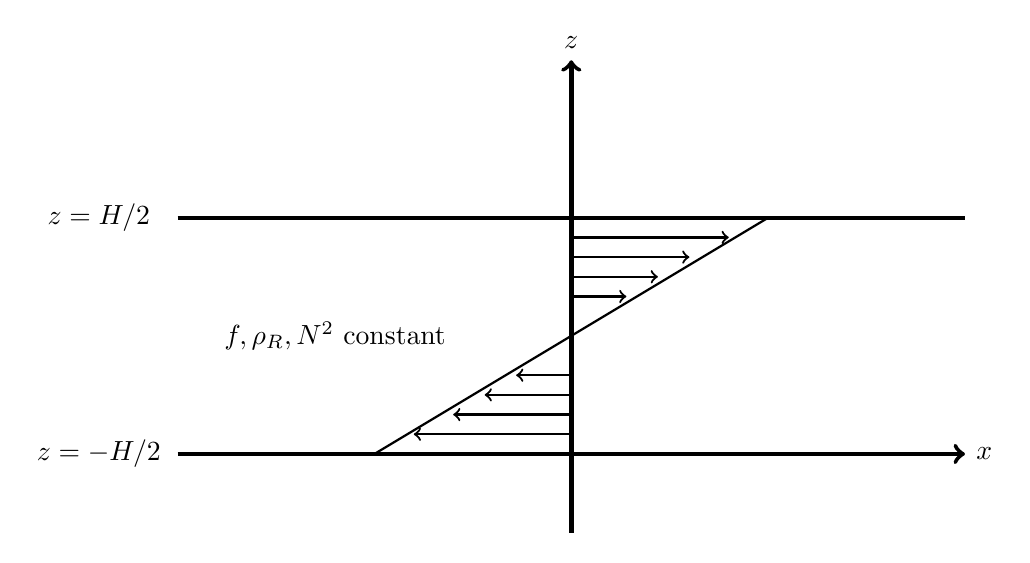
\begin{tikzpicture}
\draw[->,ultra thick] (-5,0)--(5,0) node[right]{$x$};
\draw[->,ultra thick] (0,-1)--(0,5) node[above]{$z$};
\draw[ultra thick] (-5,3)--(5,3); 
\draw[thick] (-2.5,0) -- (2.5,3);
\draw[thick,->] (0,2) -- (0.7,2);
\draw[thick,->] (0,2.25) -- (1.1,2.25);
\draw[thick,->] (0,2.5) -- (1.5,2.5);
\draw[thick,->] (0,2.75) -- (2,2.75);
\draw[thick,->] (0,1) -- (-0.7,1);
\draw[thick,->] (0,0.75) -- (-1.1,0.75);
\draw[thick,->] (0,0.5) -- (-1.5,0.5);
\draw[thick,->] (0,0.25) -- (-2,0.25);
\node at (-6,3) {$z = H/2$};
\node at (-6,0) {$z = -H/2$};
\node at (-3,1.5) {$f,\rho_R,N^2$ constant};
\end{tikzpicture}
  \caption{ }
  \label{eadyexample}
\end{figure}
\section{Cyclogenesis} 

\section{Summary}
\bibliography{references.bib}
\bibliographystyle{apa}

\end{document}
